\documentclass{article}

%% Denote paragraphs with vertical space rather than indenting (not critical)
\usepackage{parskip}

%% Support for URL in introductory text (not needed for main example)
\usepackage{url}

%% *** Enable PGFPLOTS (automatically enables TikZ) ***
\usepackage{pgfplots}

%% Prevent some PGFPLOTS messages (not critical)
\pgfplotsset{compat=1.18,compat/show suggested version=false}


\begin{document}

%% Introductory Text
Example 10.18 from the book\\
\emph{Unlocking LaTeX Graphics: A Concise Guide to Ti$k$Z/PGF and PGFPLOTS}.\\
For more information, visit \url{https://latex-graphics.com}.
\par\bigskip

%% *** START OF EXAMPLE CODE ***
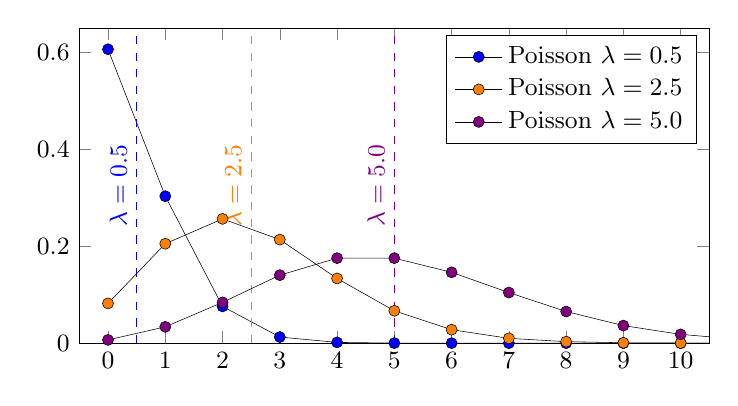
\begin{tikzpicture}
  \begin{axis} [scale only axis,
      width=8cm, height=4cm, font=\small,
      xtick=data, xmax=10, enlarge x limits=0.05, ymin=0, ymax=0.65
    ]
    \foreach \lval/\clr in {0.5/blue, 2.5/orange, 5.0/violet}
    {
      \edef\temp{
        \noexpand\addplot[\clr,very thin,mark=*,draw=black]
          expression[samples at={0,1,2,...,11}]
          {exp(-\lval)*(\lval^x)/factorial(x)};
        \noexpand\addlegendentry{Poisson $\lambda=\lval$}
        \noexpand\draw[\clr,dashed]
          (axis cs:\lval,0) -- (axis cs:\lval,0.65)
          node[midway,auto,sloped] {$\lambda=\lval$};
      }\temp
    }
  \end{axis}
\end{tikzpicture}
%% *** END OF EXAMPLE CODE ***

\end{document}
